\documentclass{article}
\usepackage[utf8]{inputenc}
\usepackage{tikz}
\usepackage{mathpazo}
\usepackage[margin=1in]{geometry}
\newcounter{row}
\newcounter{col}

\newcommand\setrow[9]{
  \setcounter{col}{1}
  \foreach \n in {#1, #2, #3, #4, #5, #6, #7, #8, #9} {
    \edef\x{\value{col} - 0.5}
    \edef\y{9.5 - \value{row}}
    \node[anchor=center] at (\x, \y) {\textbf{\fontsize{1.4cm}{1cm}\selectfont\n}};
    \stepcounter{col}
  }
  \stepcounter{row}
}

\begin{document}

\begin{titlepage}
	\centering
	{\scshape\LARGE Pouf-Pouf Production \par}
	\vspace{1.5cm}
	{\huge\bfseries Grilles de SUDOKU\par}
	\vfill
\end{titlepage}

% Add csv2tex.sh result in this space
% --- BEGIN ---

\paragraph{{\large Niveau très facile}}\mbox{} \\
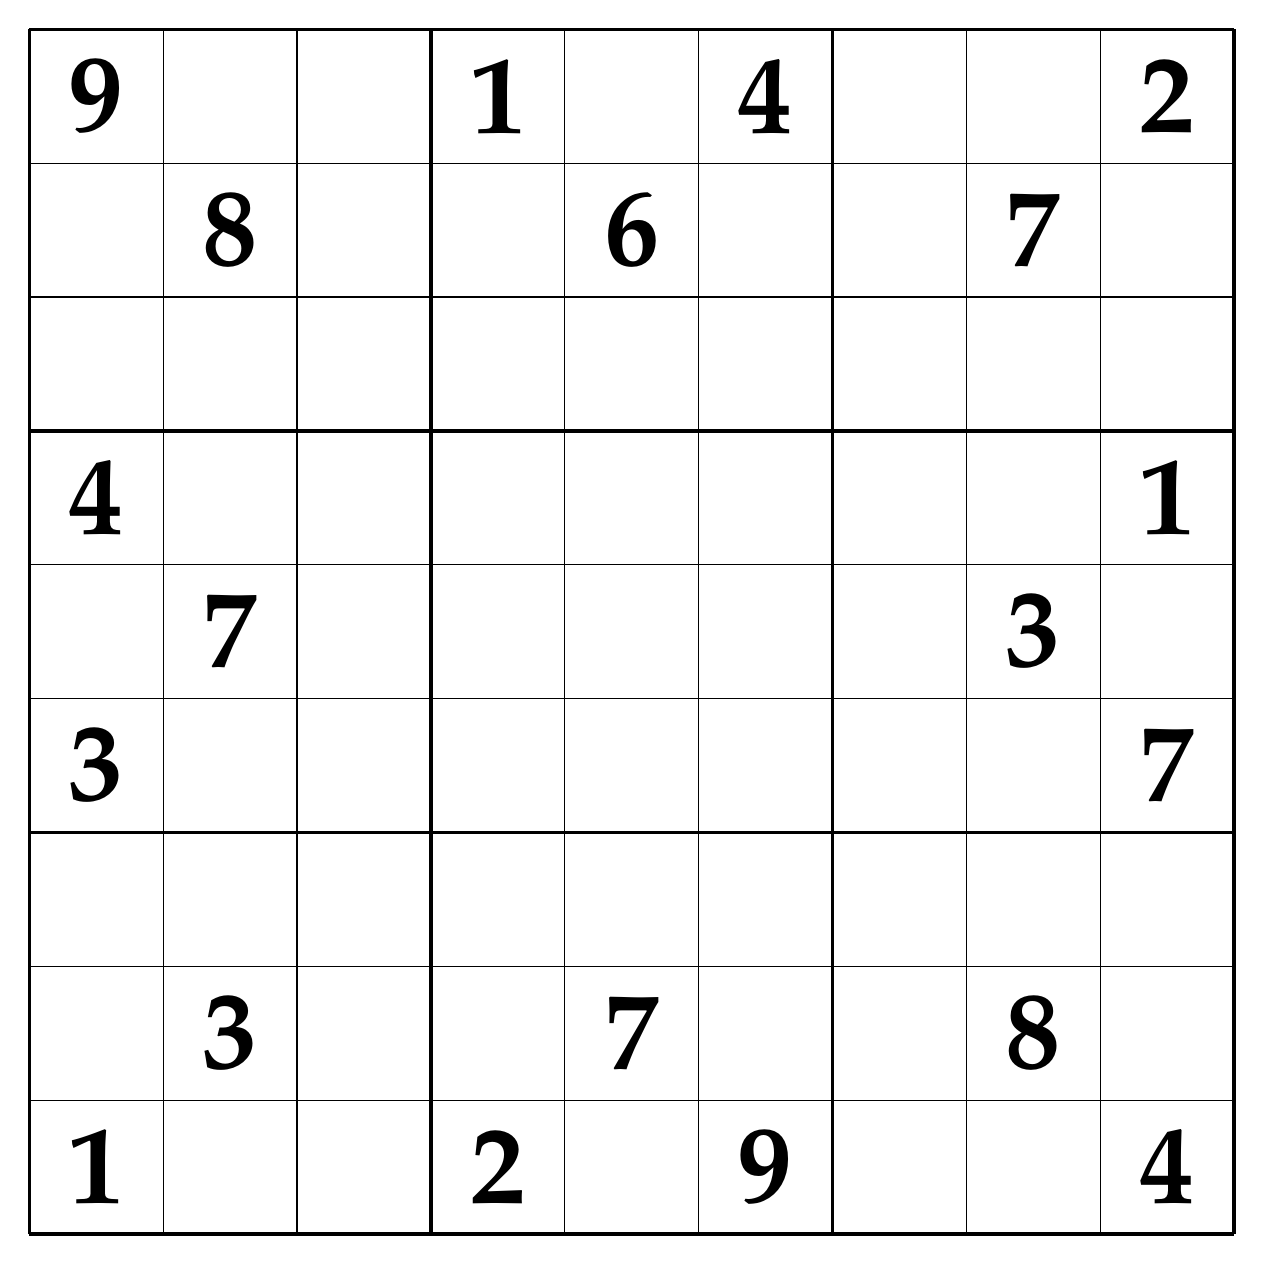
\begin{tikzpicture}[scale=1.7]
 \begin{scope}
  \draw (0, 0) grid (9, 9);
  \draw[very thick, scale=3] (0, 0) grid (3, 3);
  \setcounter{row}{1}

  \setrow {9}{ }{ }{1}{ }{4}{ }{ }{2}
  \setrow { }{8}{ }{ }{6}{ }{ }{7}{ }
  \setrow { }{ }{ }{ }{ }{ }{ }{ }{ }
  \setrow {4}{ }{ }{ }{ }{ }{ }{ }{1}
  \setrow { }{7}{ }{ }{ }{ }{ }{3}{ }
  \setrow {3}{ }{ }{ }{ }{ }{ }{ }{7}
  \setrow { }{ }{ }{ }{ }{ }{ }{ }{ }
  \setrow { }{3}{ }{ }{7}{ }{ }{8}{ }
  \setrow {1}{ }{ }{2}{ }{9}{ }{ }{4}

 \end{scope}
\end{tikzpicture}
\newpage

% --- END ---

\end{document}

